\begin{question}[type=exam] (\addpoints{10}) %pontuação da questão %caso queira que o enunciado tenha o nome "Exercício 1." e não "Questão", apague o a configuração [type=exam].
A figura~\ref{fig:graf1} representa o gráfico de uma função polinomial do 2º grau, escreva a função de descreve seu comportamento:

    \begingroup %adicionar imagem na questão, graficos e afins.
        \centering
        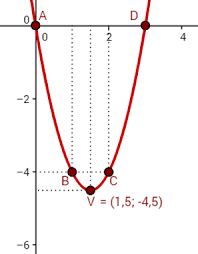
\includegraphics[width=0.4\linewidth ,height=0.4\linewidth]{graf1.png}
        \captionof{figure}{Gráfico de função}\label{fig:graf1}
    \endgroup

%\begin{tasks}(1)
 %       \task $x^2-1=2$
  %      \task $7x-1=0$
   %     \task $2x^2-2=0$   
%    \end{tasks}
\end{question}


   